\documentclass[a4paper]{article}
\usepackage{geometry}
\geometry{left=3.5cm,right=3.5cm,top=3.5cm,bottom=3.5cm}
\usepackage{amsmath, amssymb}
\usepackage{graphicx}
\usepackage{subfigure}
\usepackage{pdfpages}
\usepackage{multirow}

\usepackage{xeCJK}
\setmainfont{Times New Roman}
\setCJKmainfont[BoldFont=SimHei,ItalicFont=KaiTi]{SimSun}

\usepackage{indentfirst}
\setlength{\parindent}{2em}

\usepackage{fancyhdr}
\pagestyle{fancy}
\usepackage{lastpage}
\rhead{}
\lhead{}
\cfoot{\thepage{}}
\renewcommand{\headrulewidth}{0pt}
\renewcommand{\figurename}{图}
\renewcommand{\tablename}{表}
\renewcommand{\abstractname}{摘要}
\renewcommand{\contentsname}{\CJKfamily{SimHei} 目录}

\headheight 14pt

\usepackage{float}

\renewcommand\baselinestretch{1.2}

\begin{document}

\begin{titlepage}


\includepdf[pages=2-3,offset=0cm 0cm]{title.pdf}

\end{titlepage}

\begin{Huge}
	\centering{\textbf{ATM 交易状态特征分析与异常检测}}
\end{Huge}
\begin{large}
	\begin{flushright}
		
	\end{flushright}
\end{large}
\ \ \\\\

\begin{abstract}
\textit{}
\end{abstract}

\newpage

\tableofcontents

\newpage

\part{引言}
近些年来,由于人民生活水平的提高,银行的业务量飞速提升。与此同时也带了取款存款难的问题。
为了解决这个问题,近几年许多银行都开始广泛使用 ATM 自动取款机,并建立了一套 ATM 交易系统。
但是由于各种原因, ATM 交易系统有时会发上故障,影响银行的工作效率。
因此,为了实时掌握全行的业务状态,及时发现故障,银行总行数据中心监控系统每分钟会对各分行的交易信息进行汇总统计。
汇总信息包括业务量、交易成功率、交易响应时间三个指标。
监控系统要从这三个指标的变化情况中及时发现 ATM 交易系统是否出现故障。
本文就如何从这三个指标的变化情况及时发现交易系统的故障做了理论分析,并用所给数据进行了模拟,得到了相对精准的预报。

\part{表征业务状态的特征参量}
\begin{figure}[htbp]
	\centering
	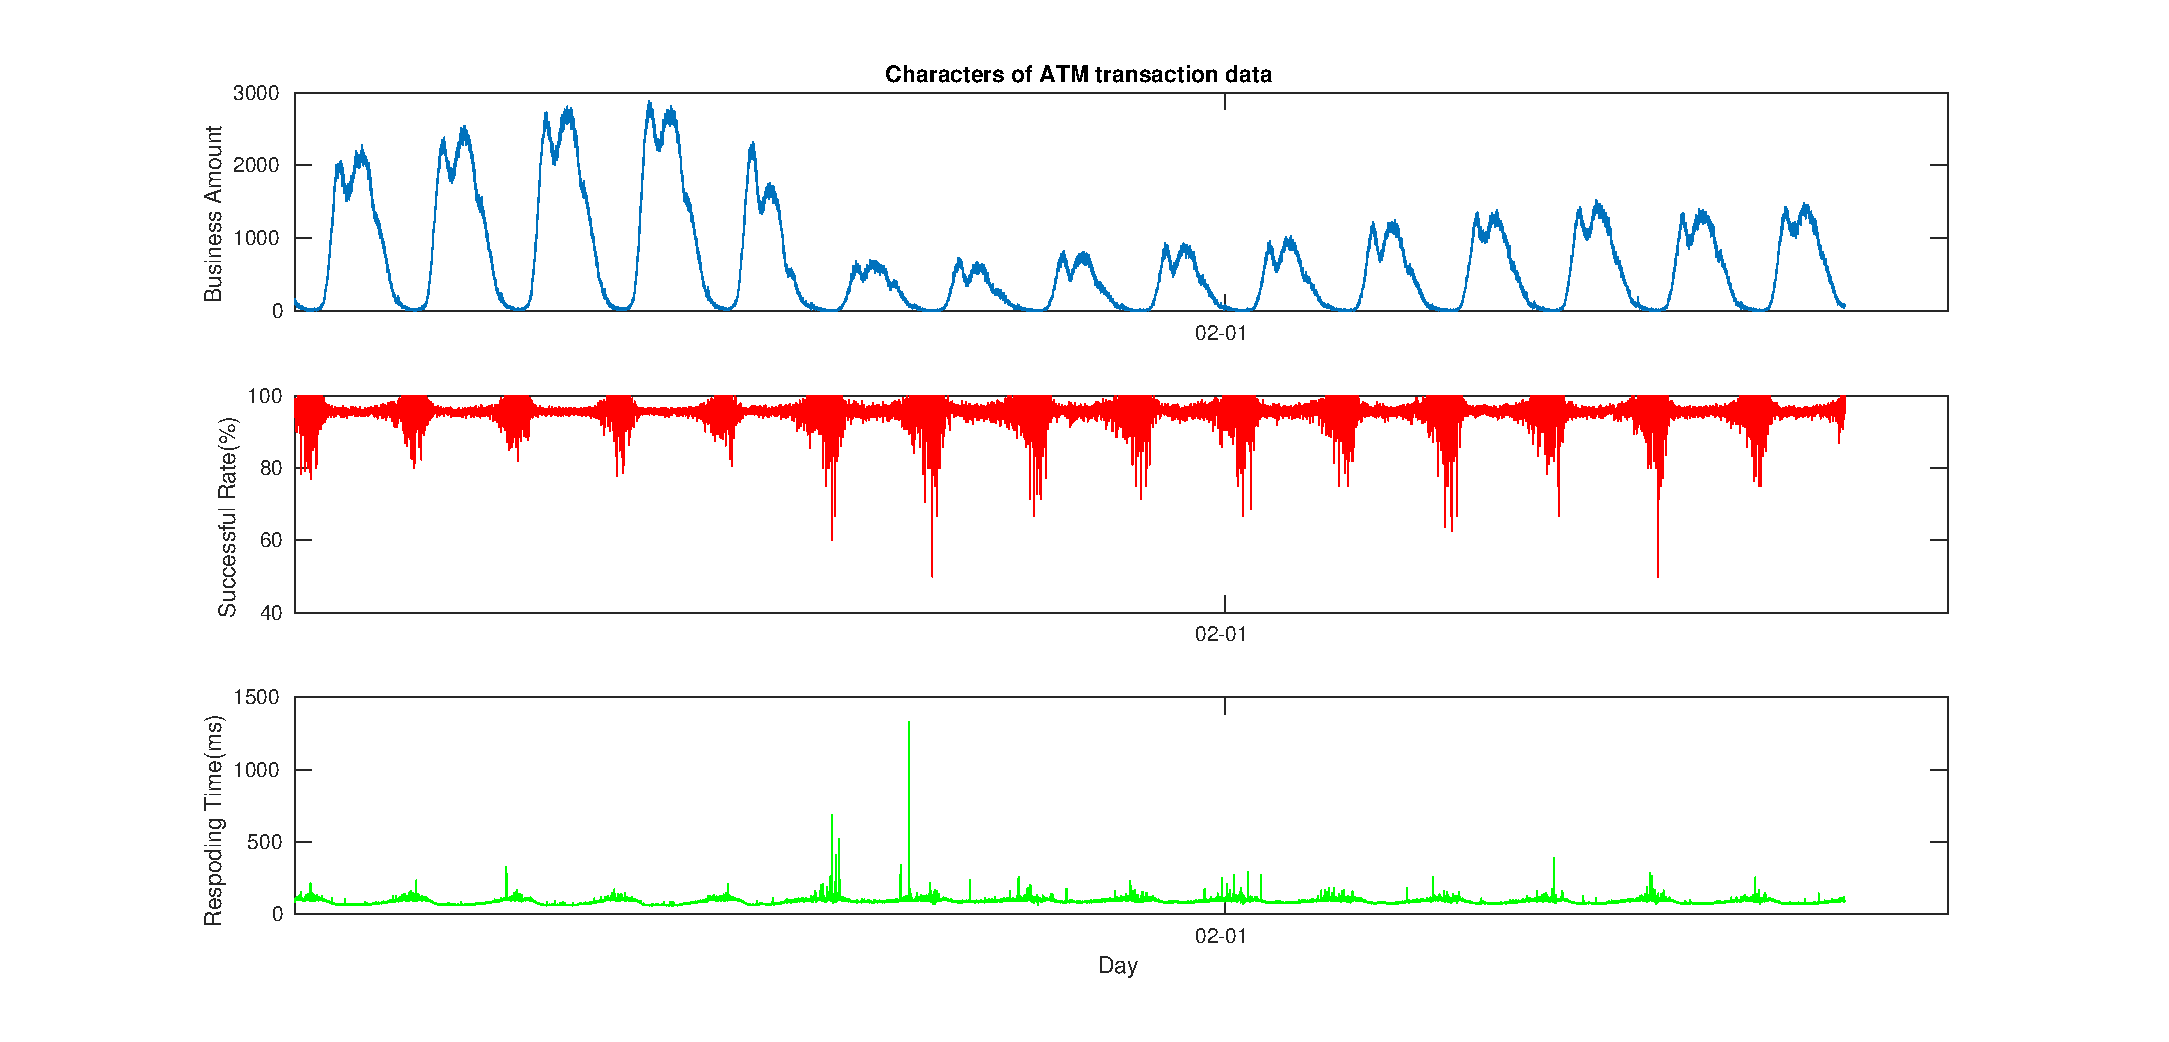
\includegraphics[scale=0.4]{pic/jan-feb-bsr.eps}
	\caption{ATM交易状态变化}
     \label{fig:char}
\end{figure}
ATM 业务状态随着时间是不断变化的;这种变化不仅仅是发生在每一天之内,同时也是存在于相邻两天的差异中。
通过对图 \ref{fig:char} 的观察可知,业务状态呈现以天为单位的周期变化,每一天的曲线大致相似但是有所区别。
为了在最少的特征参量下尽可能准确地描述业务状态的变化,我们可以通过将每一天的数据按时间划分成不同的模式。
对于每一种模式,我们会采用不同的特征参量来描述,这些特征参量在每个时间段内具有一定的稳定性。
\\
\section*{记号表}
\begin{table}[H]
	\centering
	\caption{}
	\label{tab:problem1_symbols}
	\begin{tabular}{ccc}
		\hline
		符号 & 含义 & 备注 \\
		\hline
		$t$ & Time & \\
        $B(t)$ & 业务量 & $[t, t+1)$ 内的累计业务量 \\
		$S(t)$ & 成功率 & $[t, t+1)$ 内的平均成功率 \\
		$R(t)$ & 响应时间 & $[t, t+1)$ 内的平均响应时间 \\
		$M_T^i$ & 中位数 & $T \in \{B, S, R\}$ \\
        $\sigma_T^i$ & 标准差 & $i \in \{1, 2, 3, 4\}$ \\
		$\tilde{\sigma}_T^i$ & 带修正的标准差 & 剔除原数据中落在 $c \cdot \sigma_T^i$ 外之后重新计算得到 \\
		$\vartheta_B^i$ & 斜率 & \\
        $r_B^i$ & 相关系数 & 最小二乘法拟合第 2、4 个时间段的相关系数\\
		\hline
	\end{tabular} \\
\end{table}
通过对数据的分析,总的来说,$B(t)$,$S(t)$,$R(t)$ 对于时间 $t$ 大致呈周期分布,且在每一个周期内的不同时间段会显示出不同的模式。
为了描述这些模式,我们主要通过中位数 $M$ ,标准差 $\sigma_T^i$ (与带有修正的标准差 $\tilde{\sigma}_T^i$ ) ,斜率 $\vartheta_B^i$ 这些特征参量来表征不同的状态。
\\
值得注意的是,我们可以很明显地从图 \ref{fig:char} 中看出一月份的业务量数据波动是非常大的。
由于一月底春节的影响,银行的业务量呈现与平日不同的模式,对于参数的估计是不利的,因此\emph{下文进行参数计算时选择的是二月至四月的数据}。

\section{业务量的特征参数}
\indent 业务量是指总行接收到的支行业务总数。
对于业务量 $B(t)$ ,我们将一天划分成四个时段,即:6 $\sim$ 9点,9 $\sim$ 18点,18 $\sim$ 23点,以及23 $\sim$ 次日6点,可参见图 \ref{fig:char_feb-1}。
对于每一个时段,业务量都有一些鲜明的特征,数据参见表 \ref{tab:char_B} 。
\begin{table}[H]
	\centering
	\caption{业务量特征参数}
	\label{tab:char_B}
	\begin{tabular}{c|cc|c|c|cc|cc}
		\hline
		\multirow{2}{*}{时间段 $i$} & \multicolumn{2}{c}{$M_B^i$} & $\sigma_B^i$ & $\tilde{\sigma}_B^i$ & \multicolumn{2}{c}{$\vartheta_B^i$} & \multicolumn{2}{c}{$r_B^i$} \\
		& mean         & sd           & mean        & mean                 & mean             & sd               & mean         & sd           \\
		\hline
		6-9 1                    & 406.73       & 121.87       & 289.16      & 286.19               & 5.4751           & 0.80011          & 0.98275      & 0.011052     \\
        9-18 2                   & 1053.9       & 108.17       & 102.34      & 96.315               & -$^{(*)}$     & -                & -            & -            \\
		18-23 3                  & 558.95       & 95.123       & 274.21      & 273.8                & -3.134           & 0.50446          & -0.9896      & 0.002531     \\
		23-(6) 4                 & 27.744       & 3.8689       & 29.158      & 23.813               & -                & -                & -            & -           \\
		\hline
	\end{tabular}
\end{table}
(*) \emph{对于日间与夜间业务量稳定的模式,其斜率没有显著的含义,因此未计算斜率与相关系数。}
\begin{figure}[htbp]
	\centering
	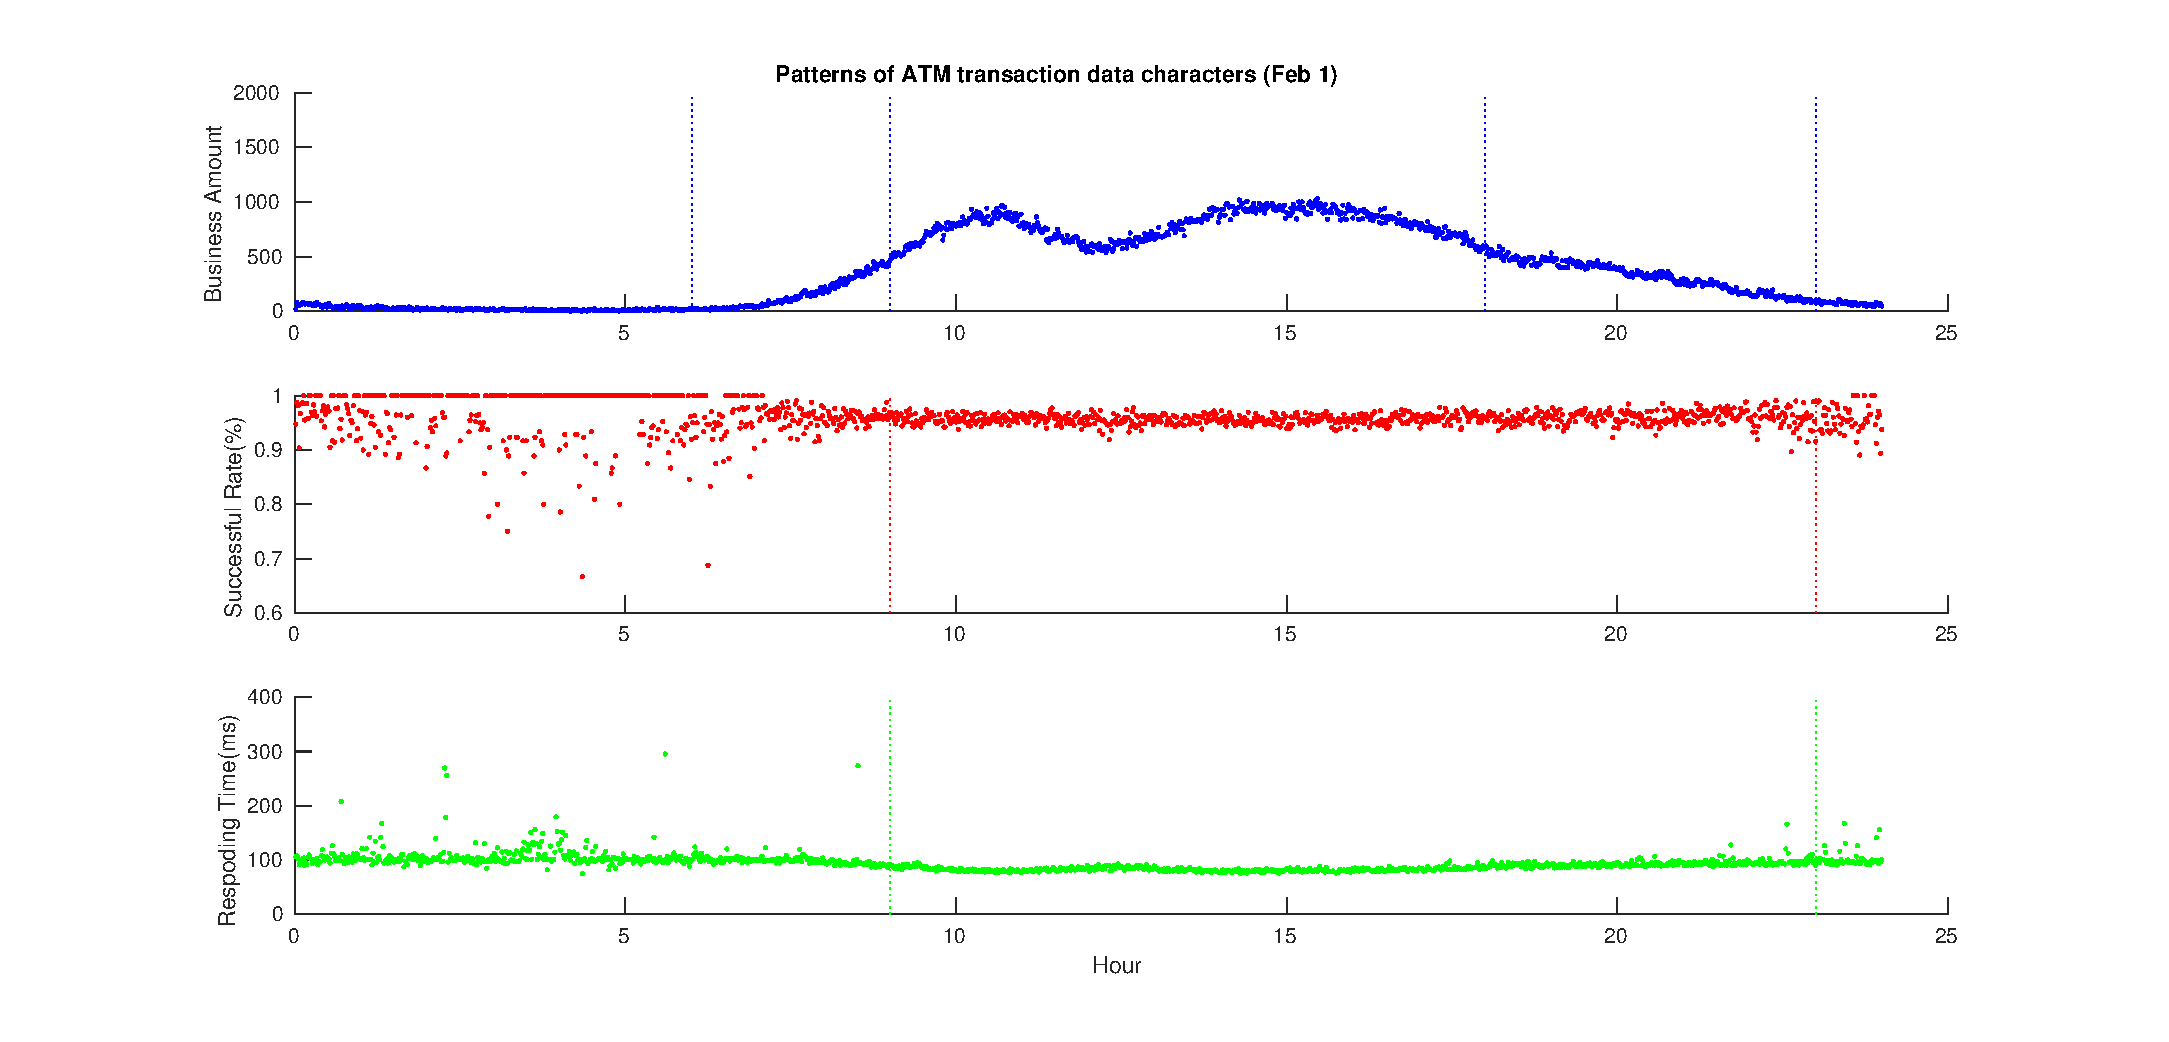
\includegraphics[scale=0.4]{pic/feb-1-bsr-pattern.eps}
	\caption{业务量、成功率、响应时间的典型分布}
    \label{fig:char_feb-1}
\end{figure}
\begin{itemize}
    \item 对于 6 $\sim$ 9 点,是业务量上升阶段,这个时段,平均值的意义不是很明显,这里我们用其上升的速度,也即斜率 $\vartheta_B^1$ 来表征这一时段的特点。
    \item 9 $\sim$ 18 点是一天中业务最为繁忙的一个时期。业务量大,同时波动的幅度也比较明显。所以,这段时间内中位数 $M_B^2$ 较大,标准差 $\sigma_B^2$ 也很大
    \item 第三个时间段是 18 $\sim$ 23 点,这段时间是业务下降阶段。与 6 $\sim$ 9 点类似,我们也用斜率 $\vartheta_B^3$来记录这一时期的特征。
    \item 对于 23 $\sim$ 次日 6 点,由于是夜间,客户往往不会选择在这段时间办理业务。所以业务量较少,波动不明显,从而 $M_B^4$ 和 $\sigma_B^4$ 都比较小。
\end{itemize}
进一步的,通过对比每一天的业务量的这些特征参量,我们发现每一天的趋势基本相同,即每一天这四个时段的趋势基本相同。
但具体到数值上时,有较大的偏差。
由表 \ref{tab:char_B} 的数据可以看出,日间的中位数的标准差要远大于每日标准差的平均值。
为了降低异常点对于特征参量数值的影响,将每日偏离中位数 $c$ 倍标准差外的数据予以剔除,并重新求标准差,得到表 \ref{tab:char_B} 第五列 $\tilde{\sigma}_B^i$ 的数据。
\\
\indent 对业务量异常点的出现原因,我们有以下分析:业务量是指总行接收到的支行业务总数。
当业务量陡然减少时,由于业务量数据是由支行节点通过网络传给总行,所以此时的故障很有可能为支行与总行的网络中断导致的。

\section{成功率的特征参数}
\indent 成功率的模式比较简单,主要分为两个时段,可参见图 \ref{fig:char_feb-1},数据参见表 \ref{tab:char_S} 。
\begin{table}[H]
	\centering
	\caption{成功率特征参数}
	\label{tab:char_S}
	\begin{tabular}{c|cc|c|c}
		\hline
		\multirow{2}{*}{时间段 $i$} & \multicolumn{2}{c}{$M_S^i$} & $\sigma_S^i$ & $\tilde{\sigma}_S^i$ \\
		& mean        & sd            & mean        & mean                 \\
		\hline
		9-23 1                   & 0.95683     & 0.00097769    & 0.0092547   & 0.0074817            \\
		23-(9) 2                 & 0.96463     & 0.0022323     & 0.0394      & 0.027581            \\
		\hline
	\end{tabular}
\end{table}
9 点至 23 点业务量繁多,银行后台的稳定性要求很高,所以这段时间的成功率的标准差比较小。
而 23 点至次日 9 点这段时间,由于这段时间业务量少,所以银行的通讯线路会非常通畅。
但另一方面,也由于业务较少,银行后台要求的稳定性有所降低;
考虑到银行的机器或者程序的检修一般都在晚上进行,不确定因素增加,所以这个时间段数据相对比较分散,标准差 $\sigma_S^2$ 很大,有时成功率能达到 100\% ,有时则会很低。
\\
\indent 影响交易的成功与否的因素很多,比如分行的数据变更或者配置错误、总行的数据中心后端处理系统应用进程异常等等。
若出现上述错误时,就会导致交易成功率下降。所以当成功率出现异常点时,应该及时检查是否这几个地方出现了问题。


\section{响应时间的特征参数}
\indent 响应时间的模式也主要分为两个时段,可参见图 \ref{fig:char_feb-1},数据参见表 \ref{tab:char_R} 。
\begin{table}[H]
	\centering
	\caption{响应时间特征参数}
	\label{tab:char_R}
	\begin{tabular}{c|cc|c|c}
		\hline
		\multirow{2}{*}{时间段 $i$} & \multicolumn{2}{c}{$M_S^i$} & $\sigma_S^i$ & $\tilde{\sigma}_S^i$ \\
		& mean        & sd            & mean        & mean                 \\
		\hline
		9-23 1                   & 83.212     & 9.0861    & 16.031   & 5.8181            \\
		23-(9) 2                 & 100.72     & 7.9057     & 194.53      & 17.266            \\
		\hline
	\end{tabular}
\end{table}
从 9 点至 23 点业务量巨大,银行必须使用大量的服务器才能满足客户业务量的需求,同时还要尽量减少响应时间以获得更多的业务量。
而对于 23 点至次日 9 点则相反,由于业务量较少,所以即使响应时间较慢也不会影响银行的处理效率;
同时出于降低能耗的原因,银行很有可能会减少夜间服务器的数量,从而使得这期间的响应时间 $R(t)$ 的中位数较大。
\\
\indent 响应时间主要受到总行数据中心后台处理系统的影响。
当处理系统异常,比如CPU负荷过大时,就会导致交易处理过程缓慢,进而导致响应时间过长。

\section*{小结}
通过上面的讨论,我们对这三项指标反应的 ATM 交易状态特性有了初步的了解,提取出了每个指标的特征参数,并对每个指标中出现奇异点的原因进行了分析。

\part{基于SSA算法的含噪声时间序列预测}
\section{引述}
\indent 通过分析数据,我们发现交易状态关于时间有明显的周期性趋势,但在不同的周期中,也有一些差异。
要找出异常点,从来理论上来说,就是要找到一个对三个指标进行预测的模型,并将实际值与预测值相比较;
当误差超过预先设定的阈值时,我们就认为出现了异常点。
经过比较不同算法的优劣,我们最终采用了SSA算法作为我们的预测算法。
\\
\indent 对于我们研究的这三个指标,我们可以将它们看成是一串时间序列 $F=(f_0, f_1, \cdots, f_{N-1})$ ,其中 $f \in \{B, S, R\}$ 。
$N$ 为这一时间序列的长度。
通过前面的分析,我们知道这串序列有一个弱周期 1 天 。
我们要做的就是通过目前的数据去预测短期的各项指标值。
\section*{符号表}
\begin{table}[H]
	\centering
	\caption{}
	\label{tab:ssa_symbols}
	\begin{tabular}{ccc}
		\hline
		符号 & 含义 & 备注 \\
		\hline
		$L$ & 窗口长度 & \\
		$N$ & 总样本点数量 & \\
		$f_i$ & 量 $f$ 在 时间 $t_i$ 处所取的值 & $f \in \{B, S, R\}$ \\
		$\textbf{X}$ & 轨道矩阵 & \\
		$d$ & \textbf{X} 的非零奇异值个数 & \\
		$r$ & \textbf{X} 的主要成分奇异值个数 & \\
		$a_i$ & LRF 系数 & \\
		\hline
	\end{tabular} \\
\end{table}

\section{重构序列的计算}
\subsection{轨道矩阵}
首先我们按照窗口长度 $L = 1440$ 将时间序列拆为若干依次推后的小段
\begin{equation}
	\label{eqn:F_i}
	F_i = (f_{i-1}, \cdots, f_{i+L-2})^T  (1 \leq i \leq K = N - L + 1)
\end{equation}
我们将每个 $F_i$ 重新组合,得到轨道矩阵 $\textbf{X}$
\begin{equation}
	\label{eqn:X}
	\textbf{X} = (F_1, \cdots, F_K)
\end{equation}
\subsection{时间序列的奇异值分解}
我们对轨道矩阵 $\textbf{X}$ 进行奇异值分解,以得到各个不同的强度对应奇异值的贡献。
首先计算
\begin{equation}
	\label{eqn:S}
	S = \textbf{X} \textbf{X}^T
\end{equation}
实对称方阵 $S$ 有特征值 $\lambda_i$ 与对应的特征向量 $U_i$ 。
由于 $S$ 是实对称的,我们可以取合适的 $U_i$ 使得它们彼此单位正交。
\\
\indent 接下来计算 $V_i$ 以及不同奇异值对应的分解矩阵
\begin{equation}
	\label{eqn:V_i}
	V_i = \textbf{X}^T U_i / \sqrt{\lambda_i}
\end{equation}
\begin{equation}
	\label{eqn:X_i}
	\textbf{$X_i$} = \sqrt{\lambda_i} U_i V_i^T
\end{equation}
\begin{equation}
	\label{eqn:SVD_expanded}
	\textbf{X} = \Sigma_{i=1}^d \textbf{$X_i$}
\end{equation}
这里 $d$ 指轨道矩阵 $\textbf{X}$ 的非零奇异值的个数,代表的是有贡献的分解矩阵的个数,即
\begin{equation}
	\label{eqn:non-zero-char-d}
	d = max\{i \textbar \lambda_i > 0\}
\end{equation}
我们选择从大到小的前 $r$ 个奇异值作为主要的贡献项;
显然 $r < d$ 。
\subsection{时间序列的重构}
基于式 \ref{eqn:SVD_expanded} 我们可以得到轨道矩阵 $\textbf{X}$ 的 SVD 分解形式
\begin{equation}
	\label{eqn:SVD}
	\textbf{X} = \textbf{U} \Sigma \textbf{V}^T
\end{equation}
这里
\begin{equation}
	\label{eqn:SVD_U}
	\textbf{U} = (U_1, \cdots, U_K)
\end{equation}
\begin{equation}
	\label{eqn:SVD_Sigma}
	\Sigma = diag(\sqrt{\lambda_1}, \cdots, \sqrt{\lambda_K})
\end{equation}
\begin{equation}
	\label{eqn:SVD_V} 
	\textbf{V} = (V_1, \cdots, V_L)
\end{equation}
\\
\indent 于是我们就可以利用分解的结果计算 LRF 的系数。
系数 $a_i$ 由如下方法确定
\begin{align}
	\textrm{R} &= (a_{L-1}, \cdots, a_1)^T \\
	           &= \frac{1}{1-\nu^2} \Sigma_{i=1}^r \pi_i U_i^\nabla \label{eqn:R_a}
\end{align}
这里 $\pi_i$ 是向量 $U_i$ 的最后一个元素,而 $U_i^\nabla$ 是向量 $U_i$ 除去最后一个元素得到的 $(L-1)$ 维向量,并且
\begin{equation}
	\label{eqn:ssa_nu^2}
	\nu^2 = \Sigma_{i=1}^r \pi_i^2
\end{equation}

\section{预测}
至于预测的部分我们使用线性递推公式
\begin{equation}
	\label{eqn:ssa_prediction}
	\tilde{f}_N = \Sigma_{i=1}^{L-1} a_i \cdot f_{N-L+i} 
\end{equation}
作为预测的第 $(N+1)$ 个量。
为了得到之后的预测结果,我们将 $\tilde{f}_N$ 加入到原先的 $F$中,即
\begin{equation}
	\label{eqn:ssa_new_f}
	\tilde{F} = (f_0, \cdots, f_{N-1}, \tilde{f}_N)
\end{equation}
用 $\tilde{F}$ 来生成 $\tilde{X}$ ,可以计算得到 $\tilde{f}_{N+1}$ ,于是可迭代得到任意后面的一项。

\section{数值实验}
我们选取了 2 月 10  日的业务量数据,进行了上述的时间序列分析的拟合操作。
为了检验不同时间段内该算法的自适应性,我们依次选取了从 200 分钟到 1200 分钟开始的预测序列。
结果如图 \ref{fig:ssa-200-400-600} 与图 \ref{fig:ssa-800-1000-1200} 所示,误差分析列在表 \ref{tab:ssa_error} 中。
\begin{figure}[htbp]
	\centering
	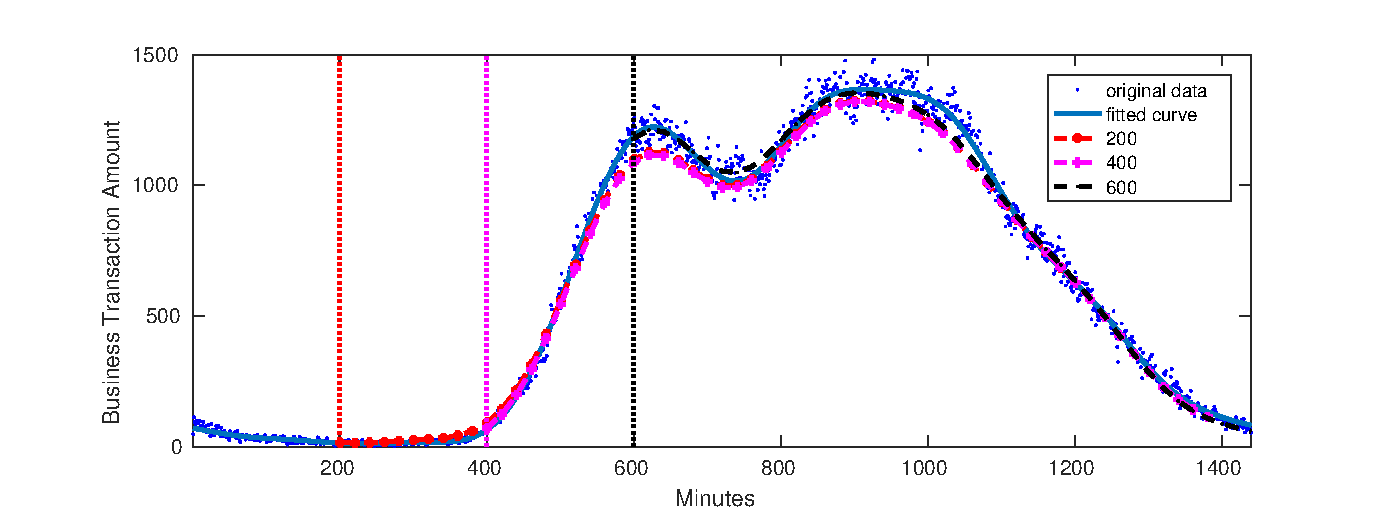
\includegraphics[scale=0.6]{pic/trade_amount_2_10_200_400_600.eps}
	\caption{对 2 月 10 日业务量进行时间序列预测 200 400 600 分钟开始}
    \label{fig:ssa-200-400-600}
\end{figure}
\begin{figure}[htbp]
	\centering
	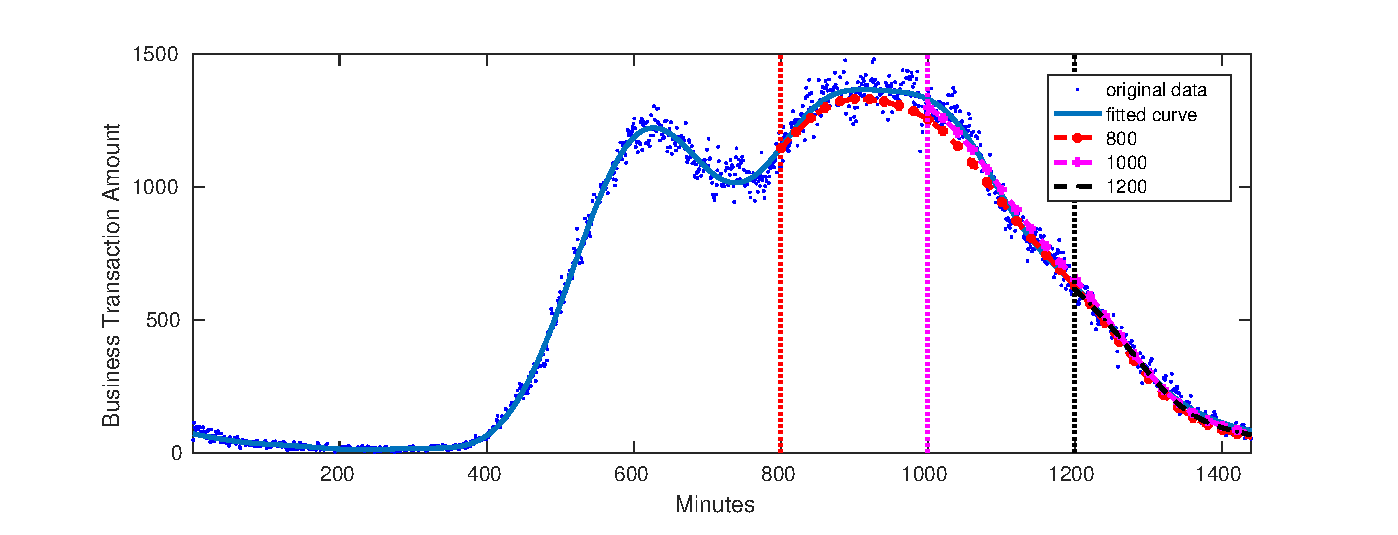
\includegraphics[scale=0.6]{pic/trade_amount_2_10_800_1000_1200.eps}
	\caption{对 2 月 10 日业务量进行时间序列预测 800 1000 1200 分钟开始}
    \label{fig:ssa-800-1000-1200}
\end{figure}
\begin{table}[htbp]
	\centering
	\caption{基于 2 月 10 日业务量进行时间序列预测的误差}
	\label{tab:ssa_error}
	\begin{tabular}{cc|ccccc}
		\hline
		开始时间(分钟) & 绝对/相对 & 20 分钟后 & 40 分钟后 & 60 分钟后 & 80 分钟后  & 100 分钟后 \\
		\hline
		200 & 绝对 & 2.889 & 4.115 & 5.494 & 6.985 & 8.780 \\
		200 & 相对 & 0.251 & 0.363 & 0.431 & 0.471 & 0.534 \\
		\hline
		400 & 绝对 & 7.231 & 7.361 & 7.361 & 7.361 & 18.273 \\
		400 & 相对 & 0.089 & 0.089 & 0.089 & 0.089 & 0.089 \\
		\hline
		600 & 绝对 & 10.043 & 10.152 & 10.152 & 10.152 & 15.296 \\
		600 & 相对 & 0.008 & 0.008 & 0.008 & 0.008 & 0.014 \\
		\hline
		800 & 绝对 & 15.960 & 26.541 & 32.615 & 34.120 & 34.121 \\
		800 & 相对 & 0.013 & 0.021 & 0.025 & 0.025 & 0.025 \\
		\hline
		1000 & 绝对 & 34.902 & 35.149 & 35.149 & 35.149 & 35.149 \\
		1000 & 相对 & 0.027 & 0.027 & 0.027 & 0.027 & 0.027 \\
		\hline
		1200 & 绝对 & 12.473 & 12.473 & 12.473 & 12.473 & 12.473 \\
		1200 & 相对 & 0.020 & 0.020 & 0.020 & 0.020 & 0.020 \\
		\hline
	\end{tabular}
\end{table}
blabla可以瞎吡吡好多呢

\section{SSA算法优化}
\indent 由于SSA算法主要是用前面的数据去预测。所以前面已知数据的质量至关重要。
而对于实际上给出的数据,往往最开始的若干个数据是比较不稳定的,因为仅由这几个数据,很难反映出此时时间序列的变化趋势。如果直接使用,会对后面的预测造成很大的影响。
为了解决这个问题,我们对SSA算法做了如下优化。\\
\indent 首先我们还是由时间序列F找出其LRF系数。接下来,由于第一个窗口$F_1$的不稳定性较大,所以我们选择从$f_1$的前k项开始进行预测,即:
\begin{equation}
f_{N-k+1}=\sum_{i=1}^{L-1}a_if_{N-L-k+i}
\end{equation}
通过上述公式不断迭代,直到$f_{N+1}$。由于选用了$f_1$前k项作为起始点,从而增加了数据中包含的时间序列的趋势信息,通过这种技巧,我们大大消除了$F_1$不稳定性的影响。下面是优化前后的拟合误差对比。可以看出优化后的算法在拟合误差上的表现总是优于改进前的表现。
\begin{figure}[htbp]
	\centering
	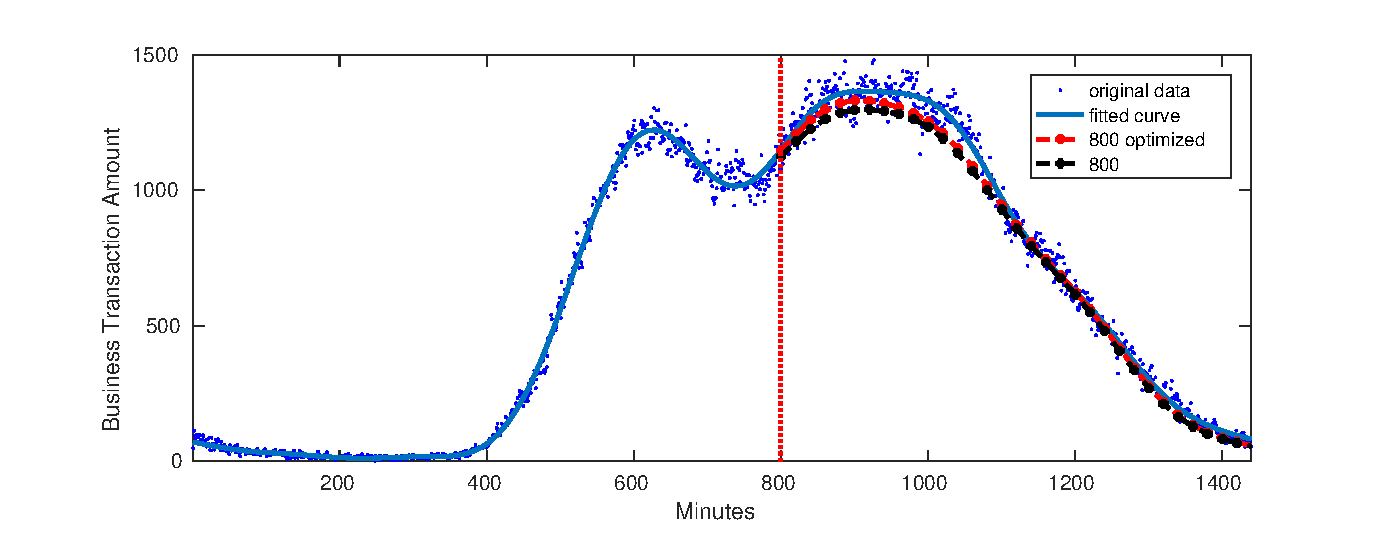
\includegraphics[scale=0.6]{pic/opt.eps}
	\caption{时间序列预测的优化改进(数据:2 月 10 日)}
  \label{fig:ssa-opt}
\end{figure}
\begin{table}[htbp]
	\centering
	\caption{时间序列预测优化改进的误差(数据:2 月 10 日)}
	\label{tab:ssa_opt_error}
	\begin{tabular}{cc|ccccc}
		\hline
		 & 绝对/相对 & 20 分钟后 & 40 分钟后 & 60 分钟后 & 80 分钟后  & 100 分钟后 \\
		\hline
		改进前 & 绝对 & 42.758 & 58.909 & 68.247 & 70.498 & 70.498 \\
		改进前 & 相对 & 0.035 & 0.046 & 0.051 & 0.052 & 0.052 \\
		\hline
		改进后 & 绝对 & 15.960 & 26.541 & 32.615 & 34.120 & 34.121 \\
		改进后 & 相对 & 0.013 & 0.021 & 0.025 & 0.025 & 0.025 \\
		\hline
	\end{tabular}
\end{table}

\part{时间序列异常检测模型}
当上述的预测步骤给出了未来一定时间的数据趋势后,我们仅需要判断真实值与预测值之间究竟是否存在显著的偏差就可以判断系统是否发生了故障。
于是我们需要给出,当真实值与预测值偏差多大的时候,前去维修的命中率与虚报率的问题。
\section{自适应带状过滤模型}
考虑一种比较简单的过滤方案:如果观测值落在了预测值的数倍标准差以外,我们就能很确定地判断这里发生了异常。
然而,对于预测值的标准差估计往往是困难的,因为正如前文指出的那样,不同时间段量表现出不同的特征,而且这些时间段的接壤的部分并不是十分清晰的,就会导致在时间段相接附近出现大量误判。
为了解决这种问题,我们可以“动态”的计算每个点处误差分布的标准差,以达到自适应的效果。
\subsection{计算步骤}
记观测到的历史时间序列为 $F=(f_0, f_1, \cdots, f_{N-1})$ ,重构序列为 $\tilde{F}=(\tilde{f}_0, \tilde{f}_1, \cdots, \tilde{f}_{N-1})$ ,预测的下一步值为 $\tilde{f}_N$ 。
为了计算真实值 $\xi$ 与预测值 $\tilde{f}_N$ 误差的标准差,我们使用 $\Delta F = F - \tilde{F} = (f_0 - \tilde{f}_0, f_1 - \tilde{f}_1, \cdots, f_{N-1} - \tilde{f}_{N-1})$ 的最后 $n_{tr}$ 项的标准差来估算,即
\begin{equation}
	\label{eqn:naive-std}
	\sigma_{exp} = standard \quad deviation \quad of \quad (f_{N-n_{tr}} - \tilde{f}_{N - n_{tr}}, \cdots, f_{N-1} - \tilde{f}_{N-1}))
\end{equation}
在取定标准 $c$ 的情况下,我们设定 $\pm c \cdot \sigma_{exp}$ 为报警阈值;
这里若取 $c = 2$ ,将会保留 $95.4\%$ 的正常状态数据;
若取 $c = 3$ ,将会保留 $99.73\%$ 的正常数据。
当然,如果一昧追求 $c$ 的值以求保留尽可能多的正常数据,将会影响到对于异常状态的检测,这一点我们将在下一节中提及。
\subsection{数值实验}
我们选取了 2 月 10 日的响应时间数据,取 $n_{tr} = 20, c = 2$ ,得到如图 \ref{} 的结果。
可以看出结果还是相当令人满意的。
\begin{figure}[htbp]
	\centering
	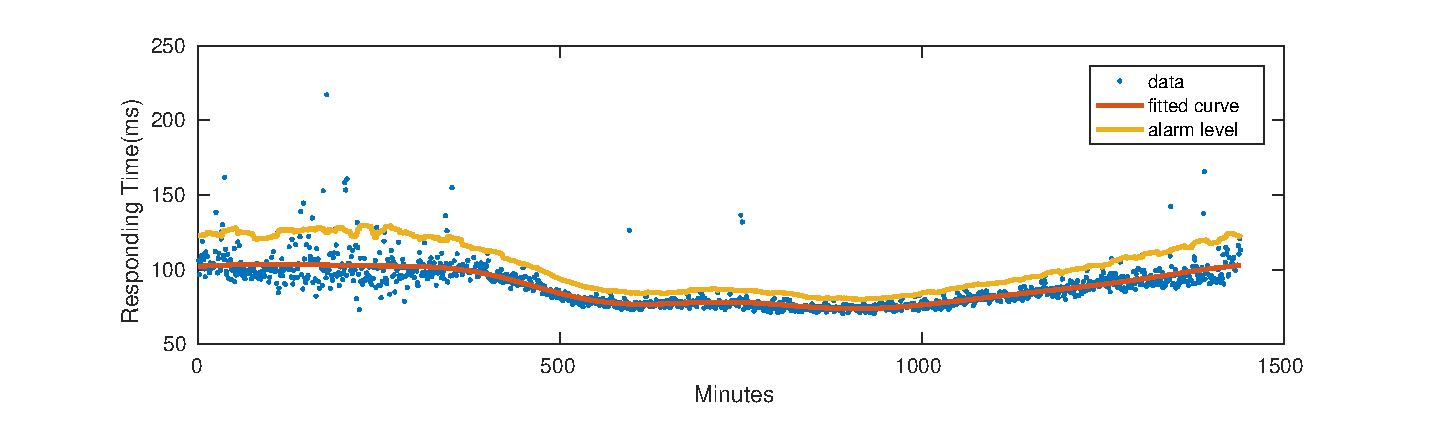
\includegraphics[scale=0.6]{pic/naive-detection.eps}
	\caption{自适应带状滤波模型结果(数据:2 月 10 日)}
  \label{fig:naive-detection}
\end{figure}

\section{信号检测理论模型}
在这部分,我们采用的理论是\footnote{Detection theory. (2017, March 25). In Wikipedia, The Free Encyclopedia. Retrieved 18:42, May 1, 2017, from https://en.wikipedia.org/w/index.php?title=Detection\_theory\&oldid=772160239}信号检测理论\footnote{Tanner Jr., Wilson P.; Higashi, M; Otsubo, R; Sakuma, T; Oyama, N; Tanaka, R; Iihara, K; Naritomi, H; Minematsu, K; John A. Swets. A decision-making theory of visual detection.. Psychological Review. 1954-11, 61 (6): 401–409 [2009-06-24]. doi:10.1037/h0058700. ISSN 0195-6108. PMID 17296997}。
考虑真实值相对于预测值发生了偏差;
这部分偏差的来源可能是来源于由于系统崩溃而导致的量的下降(或反应时间的增长),也有可能是量自身的差异性引起的。
以业务量的变化为例,当我们根据某种标准做出判断的时候,会产生四种情况:
\begin{table}[H]
	\centering
	\caption{四种可能的信号-判断状态}
	\label{tab:sdt-four}
	\begin{tabular}{|c|c|c|}
		\hline
		 & 真实值低于警报值 & 真实值高于警报值 \\
		\hline
		异常 & 击中 & 漏报 \\
		\hline
		无异常 & 虚报 & 正确否定 \\
		\hline
	\end{tabular} \\
\end{table}
我们所关心的,是在异常/无异常状态下,真实值低于警报值从而判断为有异常的概率。
我们将这两个概率命名为击中率 $p_h$ 与虚报率 $p_f$ 。
\\
\indent 当我们采用不同警报值的时候,显然,击中率与虚报率会相应发生变化。
若将这两个变量画在一个坐标图中,我们得到了 ROC 反应曲线。
为了将检测系统调节至最敏感的状态,我们取到曲线上距离理想情况(即 $p_h = 1, p_f = 0$)最靠近的一点。
在这种取法下,我们能够获得较高的击中率与较低的虚报率。
\subsection*{记号表}
\begin{table}[H]
	\centering
	\caption{}
	\label{tab:sdt_symbols}
	\begin{tabular}{ccc}
		\hline
		符号 & 含义 & 备注 \\
		\hline
		$M$ & 正常状态下量 $f$ 的期望 & \\
		$\tilde{M}$ & 异常状态下量 $f$ 的期望 & \\
		$\sigma$ & 正常状态下量 $f$ 的标准差 & \\
		$\tilde{\sigma}$ & 异常状态下量 $f$ 的标准差 & \\
		$a$ & 警报值 & \\
		$p_h$ & 击中率 & \\
		$p_f$ & 虚报率 & \\
		\hline
	\end{tabular} \\
\end{table}
\subsection{假定}
我们对于实际情况作出如下假定
\begin{itemize}
    \item 对于某一时刻 $t$ ,量 $f(t)$ 的分布服从随 $t$ 变化的正态分布 $N(M(t), \sigma^2(t))$ 。
    \item 对于某一时刻 $t$ ,量 $f$ 出现异常,异常值 $\tilde{f}(t)$ 的分布服从随 t 变化的正态分布 $N(\tilde{M}(t), \tilde{\sigma}^2(t))$ 。
    \item 异常情况与正常情况的分布是独立的。
\end{itemize}
\subsection{警报值 $a$ 的选取}
\emph{考虑在给定的时刻 $t$ ,上述提到的变量在不引起歧义的情况下略去自变量 $t$ 。}
\\
引入随机变量 $\xi$ 与 $\mu$ 来描述正常与异常状态下量 $f$ 与 $\tilde{f}$。
那么我们已经知道 $\xi$ 与 $\mu$ 服从
\begin{equation}
	\label{eqn:det_xi}
	\xi \sim N(M, \sigma^2)
\end{equation}
\begin{equation}
	\label{eqn:det_mu}
	\mu \sim N(\tilde{M}, \tilde{\sigma}^2)
\end{equation}
引入警报值 $a$ ,可求得虚报率与击中率
\begin{align}
	p_f(a) &= P\{\xi < a\} \\
		&= \Psi(\frac{a-M}{\sigma}) \label{eqn:det-p_f}
\end{align}
\begin{align}
	p_h(a) &= P\{\mu < a\} \\
		&= \Psi(\frac{a-\tilde{M}}{\tilde{\sigma}}) \label{eqn:det-p_h}
\end{align}
这里的 $\Psi(x)$ 即正态分布的分布函数
\begin{equation}
	\label{eqn:psi}
	\Psi(x) = \int_{-\infty}^{x} \frac{1}{\sqrt{2\pi}}e^{-\frac{t^2}{2}} dt
\end{equation}
\begin{figure}[htbp]
	\centering
	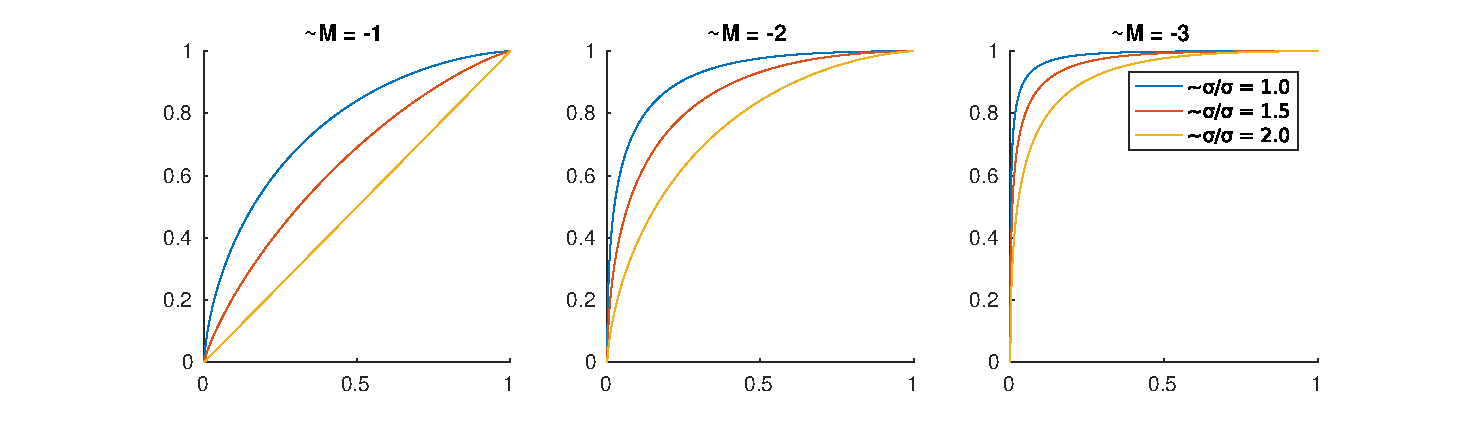
\includegraphics[scale=0.6]{pic/tilde-M-tilde-sigma.eps}
	\caption{不同程度下 ROC 反应曲线的形态}
    \label{fig:roc}
\end{figure}
观察图 \ref{fig:roc} 可见,当 $\textbar M - \tilde{M} \textbar $ 越大, $ \tilde{\sigma} / \sigma $ 越小,ROC 曲线越为敏感。
\\
关于检测系统的灵敏度,我们有数种考量标准:取 $a$ 满足
\begin{enumerate}
	\item 最小化 $\sqrt{(p_h - 1)^2 + (p_f - 0)^2}$
	\item 满足 $p_f + p_h = 1$
	\item 最大化 $p_h - p_f$
\end{enumerate}
在这里我们考虑最简单的情形,即求 $p_f + p_h = 1$ 的解。注意到恒等关系 $$\Psi(x) + \Psi(-x) = 1$$ 我们得到
\begin{equation}
	\label{eqn:det_a_formula}
	\frac{a-M}{\sigma} = -\frac{a-\tilde{M}}{\tilde{\sigma}}
\end{equation}
解得
\begin{equation}
	\label{eqn:det_a}
	a = \frac{\tilde{\sigma}M + \sigma \tilde{M}}{\tilde{\sigma} + \sigma}
\end{equation}

\subsection{对于结果的定性分析}
考察式 \ref{eqn:det_a} ,如果我们改变 $\tilde{\sigma}/\sigma$ ,相应地 $a$ 会有所改变。
\begin{itemize}
\item 如果 $\tilde{\sigma}/\sigma$ 较大,那么警报值 $a$ 将趋向于 $M$ 。这个结果的实际意义是,如果异常状态非常不确定,检测系统会比较保守,只有将低于异常值期望的值判为异常。
\item 如果 $\tilde{\sigma}/\sigma$ 较小,那么警报值 $a$ 将趋向于 $\tilde{M}$ 。这个结果的实际意义是,如果正常状态数据很不稳定,检测系统会比较激进地将低于正常值期望的值判为异常。
\end{itemize}
一般来说,异常状态总是较不稳定,因此 $\tilde{\sigma}/\sigma > 1$ ,相应地 $a$ 将更加靠近 $\tilde{M}$ 。
这与我们直观上的认识是相匹配的。
\subsection{数值实验}
表 \ref{tab:test_roc} 是 2 月 10 日的真实响应时间数据减去 SSA 拟合得到的差异结果。
\begin{table}[htbp]
	\centering
	\caption{基于 2 月 10 日响应时间数据计算的报警值 $a$}
	\label{tab:test_roc}
\begin{tabular}{c|cccc|c}
\hline
时间段 $i$  & $M$   & $\tilde{M}$ & $\sigma$ & $\tilde{\sigma}$ & $a$    \\
\hline
9-23 1   & 80.78 & 132.6        & 2.3     & $4.6^{(*)} $     & 98.05 \\
23-(9) 2 & 100.02 & 146.3        & 21.7    & 43.4             & 115.45 \\
\hline
\end{tabular}
\end{table}\\
(*) \emph{由于异常数据数量太少,获得的标准差已无意义,故用 $2 \cdot \sigma$ 近似估计。}

\part{对于方案的评估}
\section{可靠性}
\section{与其他方法的比较}
\subsection{与相邻作差法的比较}
\indent 为了找到所求序列的突变点,一个很自然的做法就是让序列中的前后项作差。
此时可以假设ATM交易系统处于正常状态时,前后项的差分小于一个阈值$\sigma$。
从而对于所有差值大于$\sigma$的差分我们就认为此时ATM交易系统出现故障。
从简单程度来看,这种方法的确简单。但是与SSA算法相比较,前后作差法就显露出一些没有解决的问题。\\
\indent 首先,由于ATM交易指标本身有随时间变化的趋势。如果单纯的以前后项的差分作为评判异常的依据,就没有排除系统自身趋势造成的影响。\\
\indent 其次,这种前后项差分的方法并不能检测出一段时间内系统均出现故障的情形。
\subsection{与傅里叶变换的比较}
\indent 在最初建立模型时,我们也考虑过用傅里叶变换来处理这一时间序列。但是经过理论分析,我们认为这种算法不适合我们要解决的问题。
\indent 对于离散傅里叶变换,我们有如下公式:
\begin{equation}
\tilde f_k=\sum_{n=0}^{N-1}e^{-i\frac{2pi}{N}nk}f_n  \quad k=1,2,\dots,N-1.
\end{equation}
然后我们可以过滤掉噪声部分,再通过傅里叶逆变换得到拟合时间序列,用于预测监测指标的数值。
但是通过上述公式可以看出,傅里叶变换会受到异常值的影响。即局部时间t处的异常偏大或偏小,会导致在周期序列中t+kT处的值也会相应的偏大或偏小。我们通过对3月27号的业务量数据进行模拟的到如下结果。
\begin{figure}[h]
	\begin{minipage}[t]{0.5\linewidth}
    \centering
    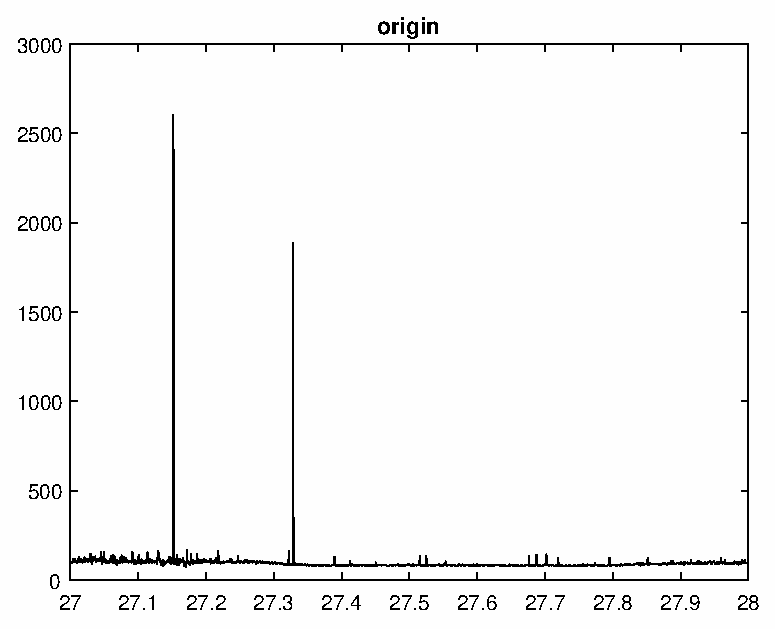
\includegraphics[scale=0.4]{pic/before_friouer.eps}
    \end{minipage}
    \begin{minipage}[t]{0.5\linewidth}
    \centering 
	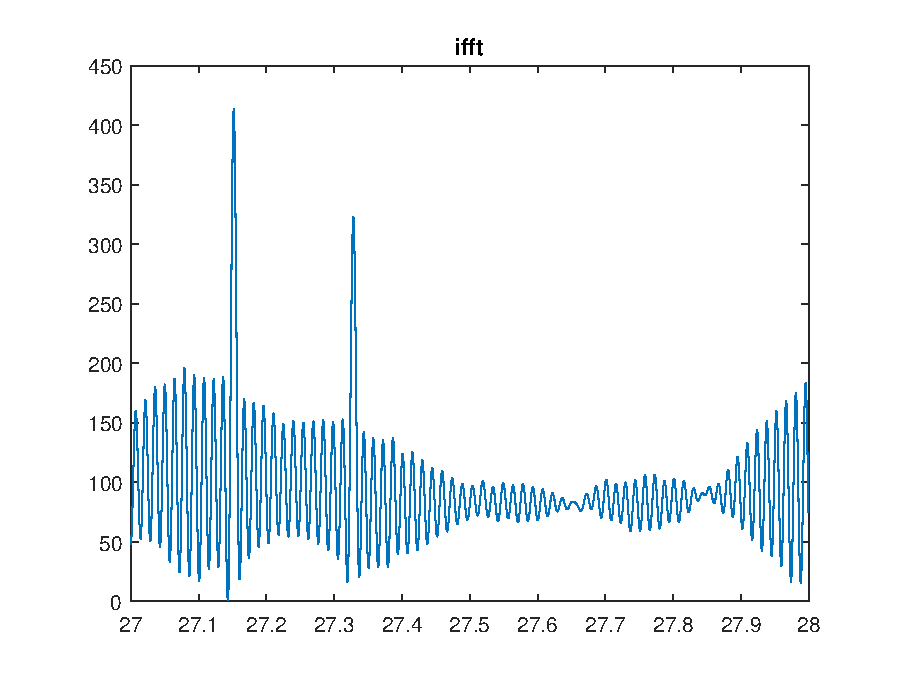
\includegraphics[scale=0.4]{pic/friouer.eps}
    \end{minipage}
	\caption{傅里叶变换处理前后的业务量图像}
     \label{fig:char}
\end{figure}
从图像可以看出变换之前的异常点严重影响了变换之后的拟合曲线。这对于我们对于指标数据的预测造成非常严重的偏差。所以使用傅里叶变换的方法是行不通的。

\part{方案的优化及完善}
\section{实际故障的监测}
\indent 在前面的模型中,我们并不知道到实际的故障是否发生。
所以在前面的处理中,我们是将重构序列作为均值,通过假设,人为的找出了警报值a.当实际值与预测值之差超过警报值a时,我们就判断系统出现故障。
这种做法没有给出实际故障与否的情况下是可以接受的。
但是缺点在于这样做的结果预报的准确率可能不是很高。 \\
\indent 所以为了优化我们的预测结果,我们希望能够测出实际的故障发生率。这样我们就可以用实际的故障发生率来计算我们设置的警报值a,从而提高命中率且减少虚报误报。
但是实际故障发生率难以直接测出。并且事实上由11节对警报值a的分析可以看出我们其实并不需要真正的测出实际故障发生率。\\
\indent 由于在实际监测过程中,发出警报后,我们可以测出实际发生故障的概率,即P(系统故障|发出警报)。而这恰恰是我们上面提到的击中率。从而我们就可以较准确地计算出警报值a的大小。
\section{后台服务器的数量}
\indent 根据前面对于检测指标的特征参数的分析,我们推测成功率以及响应时间的变化可能与后台服务器的数量相关。从已得到的数据可以大致看出后台服务器的增加可以提高系统成功率的稳定性,即可以减小成功率的标准差;同时也会降低交易的响应时间,且降低响应时间的波动。因此,当我们知道了后台服务器数量为m时,我们可以假设系统的成功率的标准差存在负线性关系,即:
\begin{equation}
\sigma=-km+b
\end{equation}
其中k>0,b均为常值。\\
这样我们可以进一步精细化我们对于警报值a的估计,从而提高击中率。	

\end{document}
